% Options for packages loaded elsewhere
\PassOptionsToPackage{unicode}{hyperref}
\PassOptionsToPackage{hyphens}{url}
%
\documentclass[
]{article}
\usepackage{amsmath,amssymb}
\usepackage{iftex}
\ifPDFTeX
  \usepackage[T1]{fontenc}
  \usepackage[utf8]{inputenc}
  \usepackage{textcomp} % provide euro and other symbols
\else % if luatex or xetex
  \usepackage{unicode-math} % this also loads fontspec
  \defaultfontfeatures{Scale=MatchLowercase}
  \defaultfontfeatures[\rmfamily]{Ligatures=TeX,Scale=1}
\fi
\usepackage{lmodern}
\ifPDFTeX\else
  % xetex/luatex font selection
\fi
% Use upquote if available, for straight quotes in verbatim environments
\IfFileExists{upquote.sty}{\usepackage{upquote}}{}
\IfFileExists{microtype.sty}{% use microtype if available
  \usepackage[]{microtype}
  \UseMicrotypeSet[protrusion]{basicmath} % disable protrusion for tt fonts
}{}
\makeatletter
\@ifundefined{KOMAClassName}{% if non-KOMA class
  \IfFileExists{parskip.sty}{%
    \usepackage{parskip}
  }{% else
    \setlength{\parindent}{0pt}
    \setlength{\parskip}{6pt plus 2pt minus 1pt}}
}{% if KOMA class
  \KOMAoptions{parskip=half}}
\makeatother
\usepackage{xcolor}
\usepackage[margin=1in]{geometry}
\usepackage{color}
\usepackage{fancyvrb}
\newcommand{\VerbBar}{|}
\newcommand{\VERB}{\Verb[commandchars=\\\{\}]}
\DefineVerbatimEnvironment{Highlighting}{Verbatim}{commandchars=\\\{\}}
% Add ',fontsize=\small' for more characters per line
\usepackage{framed}
\definecolor{shadecolor}{RGB}{248,248,248}
\newenvironment{Shaded}{\begin{snugshade}}{\end{snugshade}}
\newcommand{\AlertTok}[1]{\textcolor[rgb]{0.94,0.16,0.16}{#1}}
\newcommand{\AnnotationTok}[1]{\textcolor[rgb]{0.56,0.35,0.01}{\textbf{\textit{#1}}}}
\newcommand{\AttributeTok}[1]{\textcolor[rgb]{0.13,0.29,0.53}{#1}}
\newcommand{\BaseNTok}[1]{\textcolor[rgb]{0.00,0.00,0.81}{#1}}
\newcommand{\BuiltInTok}[1]{#1}
\newcommand{\CharTok}[1]{\textcolor[rgb]{0.31,0.60,0.02}{#1}}
\newcommand{\CommentTok}[1]{\textcolor[rgb]{0.56,0.35,0.01}{\textit{#1}}}
\newcommand{\CommentVarTok}[1]{\textcolor[rgb]{0.56,0.35,0.01}{\textbf{\textit{#1}}}}
\newcommand{\ConstantTok}[1]{\textcolor[rgb]{0.56,0.35,0.01}{#1}}
\newcommand{\ControlFlowTok}[1]{\textcolor[rgb]{0.13,0.29,0.53}{\textbf{#1}}}
\newcommand{\DataTypeTok}[1]{\textcolor[rgb]{0.13,0.29,0.53}{#1}}
\newcommand{\DecValTok}[1]{\textcolor[rgb]{0.00,0.00,0.81}{#1}}
\newcommand{\DocumentationTok}[1]{\textcolor[rgb]{0.56,0.35,0.01}{\textbf{\textit{#1}}}}
\newcommand{\ErrorTok}[1]{\textcolor[rgb]{0.64,0.00,0.00}{\textbf{#1}}}
\newcommand{\ExtensionTok}[1]{#1}
\newcommand{\FloatTok}[1]{\textcolor[rgb]{0.00,0.00,0.81}{#1}}
\newcommand{\FunctionTok}[1]{\textcolor[rgb]{0.13,0.29,0.53}{\textbf{#1}}}
\newcommand{\ImportTok}[1]{#1}
\newcommand{\InformationTok}[1]{\textcolor[rgb]{0.56,0.35,0.01}{\textbf{\textit{#1}}}}
\newcommand{\KeywordTok}[1]{\textcolor[rgb]{0.13,0.29,0.53}{\textbf{#1}}}
\newcommand{\NormalTok}[1]{#1}
\newcommand{\OperatorTok}[1]{\textcolor[rgb]{0.81,0.36,0.00}{\textbf{#1}}}
\newcommand{\OtherTok}[1]{\textcolor[rgb]{0.56,0.35,0.01}{#1}}
\newcommand{\PreprocessorTok}[1]{\textcolor[rgb]{0.56,0.35,0.01}{\textit{#1}}}
\newcommand{\RegionMarkerTok}[1]{#1}
\newcommand{\SpecialCharTok}[1]{\textcolor[rgb]{0.81,0.36,0.00}{\textbf{#1}}}
\newcommand{\SpecialStringTok}[1]{\textcolor[rgb]{0.31,0.60,0.02}{#1}}
\newcommand{\StringTok}[1]{\textcolor[rgb]{0.31,0.60,0.02}{#1}}
\newcommand{\VariableTok}[1]{\textcolor[rgb]{0.00,0.00,0.00}{#1}}
\newcommand{\VerbatimStringTok}[1]{\textcolor[rgb]{0.31,0.60,0.02}{#1}}
\newcommand{\WarningTok}[1]{\textcolor[rgb]{0.56,0.35,0.01}{\textbf{\textit{#1}}}}
\usepackage{graphicx}
\makeatletter
\def\maxwidth{\ifdim\Gin@nat@width>\linewidth\linewidth\else\Gin@nat@width\fi}
\def\maxheight{\ifdim\Gin@nat@height>\textheight\textheight\else\Gin@nat@height\fi}
\makeatother
% Scale images if necessary, so that they will not overflow the page
% margins by default, and it is still possible to overwrite the defaults
% using explicit options in \includegraphics[width, height, ...]{}
\setkeys{Gin}{width=\maxwidth,height=\maxheight,keepaspectratio}
% Set default figure placement to htbp
\makeatletter
\def\fps@figure{htbp}
\makeatother
\setlength{\emergencystretch}{3em} % prevent overfull lines
\providecommand{\tightlist}{%
  \setlength{\itemsep}{0pt}\setlength{\parskip}{0pt}}
\setcounter{secnumdepth}{-\maxdimen} % remove section numbering
\ifLuaTeX
  \usepackage{selnolig}  % disable illegal ligatures
\fi
\IfFileExists{bookmark.sty}{\usepackage{bookmark}}{\usepackage{hyperref}}
\IfFileExists{xurl.sty}{\usepackage{xurl}}{} % add URL line breaks if available
\urlstyle{same}
\hypersetup{
  pdftitle={HW\_07},
  pdfauthor={izd3},
  hidelinks,
  pdfcreator={LaTeX via pandoc}}

\title{HW\_07}
\author{izd3}
\date{}

\begin{document}
\maketitle

Use only commands \& functions that are shown in the indicated chapter
or prior chapters.

\newpage

\hypertarget{problem-01---chapter-29-exercise-01d}{%
\subsection{Problem \#01 - Chapter 29 Exercise
\#01D}\label{problem-01---chapter-29-exercise-01d}}

\begin{Shaded}
\begin{Highlighting}[]
\CommentTok{\# Show your work here}
\FunctionTok{library}\NormalTok{(scales)}
\FunctionTok{library}\NormalTok{(ggplot2)}
\end{Highlighting}
\end{Shaded}

\begin{verbatim}
## Warning: package 'ggplot2' was built under R version 4.2.3
\end{verbatim}

\begin{Shaded}
\begin{Highlighting}[]
\NormalTok{coordGraph002}\SpecialCharTok{+}\FunctionTok{coord\_fixed}\NormalTok{(}\AttributeTok{ratio=}\DecValTok{8}\SpecialCharTok{/}\DecValTok{7}\NormalTok{)}
\end{Highlighting}
\end{Shaded}

\includegraphics[height=300]{3040_HW07_izd3_files/figure-latex/unnamed-chunk-1-1}

\newpage

\hypertarget{problem-02---chapter-29-exercise-03d}{%
\subsection{Problem \#02 - Chapter 29 Exercise
\#03D}\label{problem-02---chapter-29-exercise-03d}}

\begin{Shaded}
\begin{Highlighting}[]
\CommentTok{\# Show your work here}

\NormalTok{coordGraph002}\SpecialCharTok{+}\FunctionTok{coord\_trans}\NormalTok{(}\AttributeTok{y=}\FunctionTok{sqrt\_trans}\NormalTok{(),}\AttributeTok{x=}\FunctionTok{reverse\_trans}\NormalTok{())}
\end{Highlighting}
\end{Shaded}

\includegraphics[height=300]{3040_HW07_izd3_files/figure-latex/unnamed-chunk-2-1}

\newpage

\hypertarget{problem-03---chapter-30-exercise-01d}{%
\subsection{Problem \#03 - Chapter 30 Exercise
\#01D}\label{problem-03---chapter-30-exercise-01d}}

\begin{Shaded}
\begin{Highlighting}[]
\CommentTok{\# Show your work here}
\NormalTok{facetPlot004}\SpecialCharTok{+}\FunctionTok{facet\_wrap}\NormalTok{(}\SpecialCharTok{\textasciitilde{}}\NormalTok{ggplot005.dat}\SpecialCharTok{$}\NormalTok{var}\FloatTok{.3}\NormalTok{)}
\end{Highlighting}
\end{Shaded}

\begin{verbatim}
## `stat_bin()` using `bins = 30`. Pick better value with `binwidth`.
\end{verbatim}

\includegraphics[height=300]{3040_HW07_izd3_files/figure-latex/unnamed-chunk-3-1}

\newpage

\hypertarget{problem-04---chapter-30-exercise-03d}{%
\subsection{Problem \#04 - Chapter 30 Exercise
\#03D}\label{problem-04---chapter-30-exercise-03d}}

\begin{Shaded}
\begin{Highlighting}[]
\CommentTok{\# Show your work here}
\NormalTok{facetPlot006}\SpecialCharTok{+}\FunctionTok{facet\_grid}\NormalTok{(ggplot006.dat}\SpecialCharTok{$}\NormalTok{var}\FloatTok{.3}\SpecialCharTok{\textasciitilde{}}\NormalTok{ggplot006.dat}\SpecialCharTok{$}\NormalTok{var}\FloatTok{.4}\NormalTok{)}
\end{Highlighting}
\end{Shaded}

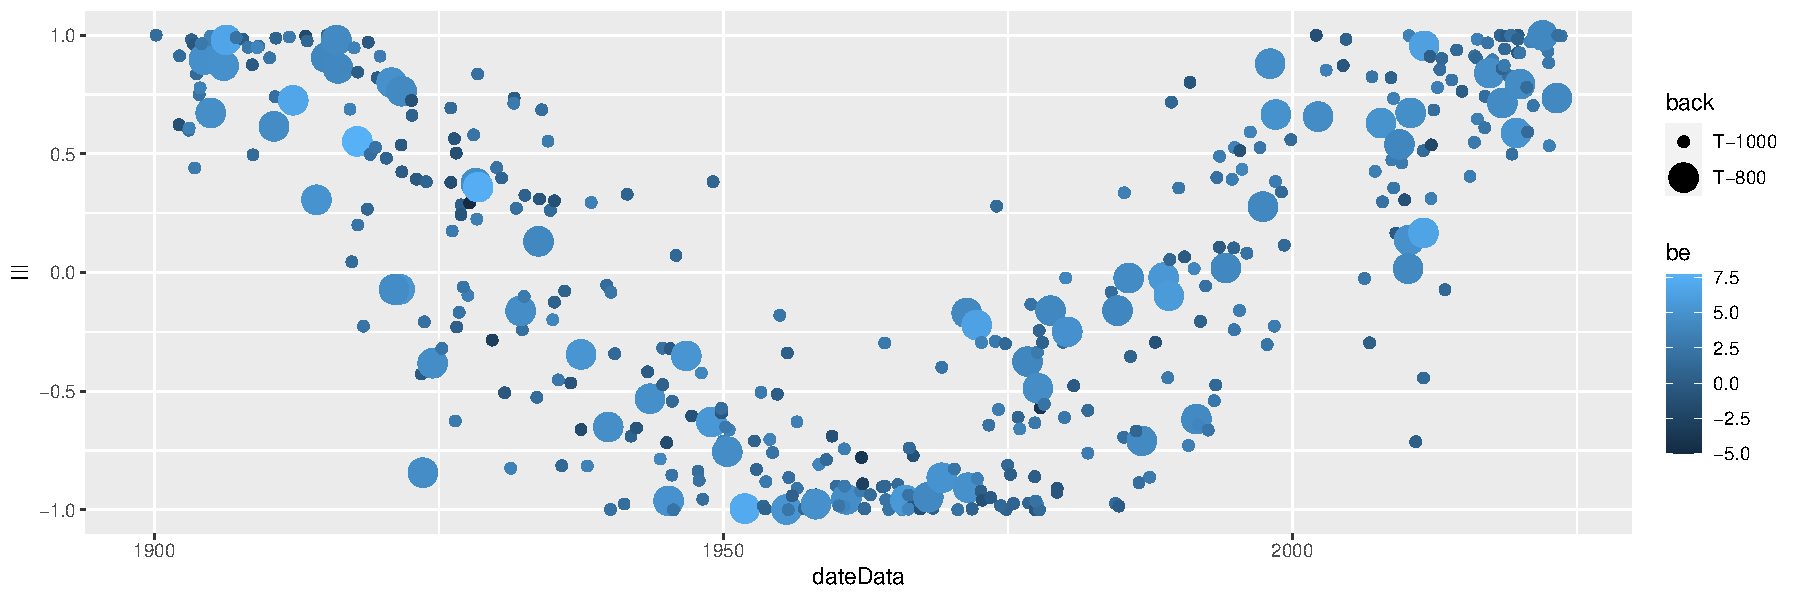
\includegraphics[height=300]{3040_HW07_izd3_files/figure-latex/unnamed-chunk-4-1}

\newpage

\hypertarget{problem-05---chapter-30-exercise-04a}{%
\subsection{Problem \#05 - Chapter 30 Exercise
\#04A}\label{problem-05---chapter-30-exercise-04a}}

\begin{Shaded}
\begin{Highlighting}[]
\CommentTok{\# Show your work here}
\NormalTok{ggplot005.dat}\SpecialCharTok{|\textgreater{}}
  \FunctionTok{ggplot}\NormalTok{(}\FunctionTok{aes}\NormalTok{(}\AttributeTok{x=}\NormalTok{var}\FloatTok{.1}\NormalTok{,}\AttributeTok{y=}\NormalTok{var}\FloatTok{.2}\NormalTok{,}\AttributeTok{color=}\NormalTok{var}\FloatTok{.3}\NormalTok{))}\SpecialCharTok{+}
  \FunctionTok{geom\_point}\NormalTok{(}\AttributeTok{shape=}\DecValTok{3}\NormalTok{,}\AttributeTok{size=}\DecValTok{4}\NormalTok{)}\SpecialCharTok{+}
  \FunctionTok{facet\_wrap}\NormalTok{(}\SpecialCharTok{\textasciitilde{}}\NormalTok{ggplot005.dat}\SpecialCharTok{$}\NormalTok{var}\FloatTok{.4}\NormalTok{)}
\end{Highlighting}
\end{Shaded}

\includegraphics[height=300]{3040_HW07_izd3_files/figure-latex/unnamed-chunk-5-1}

\newpage

\hypertarget{problem-06---chapter-31-exercise-03a}{%
\subsection{Problem \#06 - Chapter 31 Exercise
\#03A}\label{problem-06---chapter-31-exercise-03a}}

\begin{Shaded}
\begin{Highlighting}[]
\CommentTok{\# Show your work here}
\NormalTok{ggplot009.tib}\SpecialCharTok{|\textgreater{}}
  \FunctionTok{ggplot}\NormalTok{(}\FunctionTok{aes}\NormalTok{(}\AttributeTok{x=}\NormalTok{x.values,}\AttributeTok{y=}\NormalTok{y.values))}\SpecialCharTok{+}\FunctionTok{geom\_line}\NormalTok{()}
\end{Highlighting}
\end{Shaded}

\includegraphics[height=300]{3040_HW07_izd3_files/figure-latex/unnamed-chunk-6-1}

\newpage

\hypertarget{problem-07---chapter-31-exercise-04d}{%
\subsection{Problem \#07 - Chapter 31 Exercise
\#04D}\label{problem-07---chapter-31-exercise-04d}}

\begin{Shaded}
\begin{Highlighting}[]
\CommentTok{\# Show your work here}
\NormalTok{ggplot010.tib}\SpecialCharTok{|\textgreater{}}
  \FunctionTok{ggplot}\NormalTok{(}\FunctionTok{aes}\NormalTok{(}\AttributeTok{x=}\NormalTok{u.values,}\AttributeTok{y=}\NormalTok{t.values,}\AttributeTok{color=}\NormalTok{z.values))}\SpecialCharTok{+}\FunctionTok{geom\_line}\NormalTok{()}
\end{Highlighting}
\end{Shaded}

\includegraphics[height=300]{3040_HW07_izd3_files/figure-latex/unnamed-chunk-7-1}

\newpage

\hypertarget{problem-08---chapter-31-exercise-06}{%
\subsection{Problem \#08 - Chapter 31 Exercise
\#06}\label{problem-08---chapter-31-exercise-06}}

\begin{Shaded}
\begin{Highlighting}[]
\CommentTok{\# Show your work here}
\NormalTok{x}\OtherTok{\textless{}{-}}\FunctionTok{c}\NormalTok{(}\SpecialCharTok{{-}}\DecValTok{1}\NormalTok{,}\DecValTok{0}\NormalTok{,}\DecValTok{1}\NormalTok{,}\DecValTok{2}\NormalTok{,}\DecValTok{0}\NormalTok{,}\SpecialCharTok{{-}}\DecValTok{2}\NormalTok{)}
\NormalTok{y}\OtherTok{\textless{}{-}}\FunctionTok{c}\NormalTok{(}\DecValTok{0}\NormalTok{,}\DecValTok{0}\NormalTok{,}\DecValTok{0}\NormalTok{,}\DecValTok{1}\NormalTok{,}\DecValTok{1}\NormalTok{,}\DecValTok{1}\NormalTok{)}
\NormalTok{x\_head}\OtherTok{\textless{}{-}}\FunctionTok{c}\NormalTok{(}\DecValTok{0}\NormalTok{,}\FloatTok{0.29}\NormalTok{,}\DecValTok{0}\NormalTok{,}\SpecialCharTok{{-}}\NormalTok{.}\DecValTok{29}\NormalTok{)}
\NormalTok{y\_head}\OtherTok{\textless{}{-}}\FunctionTok{c}\NormalTok{(}\DecValTok{4}\NormalTok{,}\FloatTok{4.5}\NormalTok{,}\DecValTok{5}\NormalTok{,}\FloatTok{4.5}\NormalTok{)}
\NormalTok{head\_data}\OtherTok{\textless{}{-}}\FunctionTok{data.frame}\NormalTok{(}\AttributeTok{x.boat=}\NormalTok{x\_head,}\AttributeTok{y.boat=}\NormalTok{y\_head)}
\NormalTok{boat\_data}\OtherTok{\textless{}{-}}\FunctionTok{data.frame}\NormalTok{(}\AttributeTok{x.boat=}\NormalTok{x,}\AttributeTok{y.boat=}\NormalTok{y)}



\NormalTok{x\_values }\OtherTok{\textless{}{-}} \FunctionTok{seq}\NormalTok{(}\SpecialCharTok{{-}}\DecValTok{5}\NormalTok{, }\DecValTok{2}\NormalTok{, }\AttributeTok{length.out =} \DecValTok{1000}\NormalTok{)  }\CommentTok{\# 100}

\NormalTok{y\_values}\OtherTok{\textless{}{-}}\FunctionTok{c}\NormalTok{(}\FunctionTok{sinpi}\NormalTok{(x\_values)}\SpecialCharTok{/}\DecValTok{2}\NormalTok{,}\FunctionTok{sinpi}\NormalTok{(x\_values)}\SpecialCharTok{/}\FloatTok{2.7}\NormalTok{,}\FunctionTok{sinpi}\NormalTok{(x\_values)}\SpecialCharTok{/}\DecValTok{6}\NormalTok{,}\FunctionTok{sinpi}\NormalTok{(x\_values)}\SpecialCharTok{/}\DecValTok{3}\NormalTok{,}
            \FunctionTok{sinpi}\NormalTok{(x\_values)}\SpecialCharTok{/}\DecValTok{7}\NormalTok{)}

\NormalTok{x\_values}\OtherTok{\textless{}{-}}\FunctionTok{rep.int}\NormalTok{(x\_values,}\AttributeTok{times =} \DecValTok{5}\NormalTok{)}
\NormalTok{z\_values}\OtherTok{\textless{}{-}}\FunctionTok{rep}\NormalTok{(}\FunctionTok{c}\NormalTok{(}\StringTok{\textquotesingle{}A\textquotesingle{}}\NormalTok{,}\StringTok{\textquotesingle{}B\textquotesingle{}}\NormalTok{,}\StringTok{\textquotesingle{}C\textquotesingle{}}\NormalTok{,}\StringTok{\textquotesingle{}D\textquotesingle{}}\NormalTok{,}\StringTok{\textquotesingle{}E\textquotesingle{}}\NormalTok{),}\AttributeTok{each=}\DecValTok{1000}\NormalTok{)}

\NormalTok{ wavy}\OtherTok{\textless{}{-}}\FunctionTok{data.frame}\NormalTok{(}\AttributeTok{x.boat=}\NormalTok{x\_values,}\AttributeTok{y.boat=}\NormalTok{y\_values,}\AttributeTok{z.wave=}\NormalTok{z\_values)}




\FunctionTok{ggplot}\NormalTok{()}\SpecialCharTok{+}\FunctionTok{geom\_polygon}\NormalTok{(}\AttributeTok{data=}\NormalTok{boat\_data,}\AttributeTok{mapping =} \FunctionTok{aes}\NormalTok{(}\AttributeTok{x=}\NormalTok{x.boat,}\AttributeTok{y=}\NormalTok{y.boat),}
                      \AttributeTok{color=}\StringTok{\textquotesingle{}red\textquotesingle{}}\NormalTok{,}\AttributeTok{fill=}\StringTok{\textquotesingle{}red\textquotesingle{}}\NormalTok{)}\SpecialCharTok{+}
    \FunctionTok{geom\_line}\NormalTok{(}\AttributeTok{mapping =} \FunctionTok{aes}\NormalTok{(}\AttributeTok{x=}\DecValTok{0}\NormalTok{,}\AttributeTok{y=}\DecValTok{2}\SpecialCharTok{:}\DecValTok{4}\NormalTok{))}\SpecialCharTok{+}
    \FunctionTok{geom\_line}\NormalTok{(}\AttributeTok{mapping =} \FunctionTok{aes}\NormalTok{(}\AttributeTok{x=}\FunctionTok{c}\NormalTok{(}\DecValTok{0}\NormalTok{,}\DecValTok{1}\NormalTok{),}\AttributeTok{y=}\FunctionTok{c}\NormalTok{(}\DecValTok{2}\NormalTok{,}\DecValTok{1}\NormalTok{)))}\SpecialCharTok{+}
    \FunctionTok{geom\_line}\NormalTok{(}\AttributeTok{mapping =} \FunctionTok{aes}\NormalTok{(}\AttributeTok{x=}\FunctionTok{c}\NormalTok{(}\DecValTok{0}\NormalTok{,}\SpecialCharTok{{-}}\DecValTok{1}\NormalTok{),}\AttributeTok{y=}\FunctionTok{c}\NormalTok{(}\DecValTok{2}\NormalTok{,}\DecValTok{1}\NormalTok{)))}\SpecialCharTok{+}
    \FunctionTok{geom\_line}\NormalTok{(}\AttributeTok{mapping =} \FunctionTok{aes}\NormalTok{(}\AttributeTok{x=}\FunctionTok{c}\NormalTok{(}\DecValTok{0}\NormalTok{,}\FloatTok{1.5}\NormalTok{),}\AttributeTok{y=}\FunctionTok{c}\NormalTok{(}\FloatTok{3.98}\NormalTok{,}\DecValTok{3}\NormalTok{)))}\SpecialCharTok{+}
    \FunctionTok{geom\_line}\NormalTok{(}\AttributeTok{mapping =} \FunctionTok{aes}\NormalTok{(}\AttributeTok{x=}\FunctionTok{c}\NormalTok{(}\DecValTok{0}\NormalTok{,}\SpecialCharTok{{-}}\FloatTok{1.5}\NormalTok{),}\AttributeTok{y=}\FunctionTok{c}\NormalTok{(}\FloatTok{3.98}\NormalTok{,}\DecValTok{3}\NormalTok{)))}\SpecialCharTok{+}
    \FunctionTok{geom\_point}\NormalTok{(}\FunctionTok{aes}\NormalTok{(}\AttributeTok{x=}\DecValTok{0}\NormalTok{,}\AttributeTok{y=}\FloatTok{4.28}\NormalTok{),}\AttributeTok{size=}\DecValTok{20}\NormalTok{)}\SpecialCharTok{+}
    \FunctionTok{geom\_line}\NormalTok{(}\AttributeTok{data=}\NormalTok{wavy,}\AttributeTok{mapping =} \FunctionTok{aes}\NormalTok{(}\AttributeTok{x=}\NormalTok{x.boat,}\AttributeTok{y=}\NormalTok{y.boat,}\AttributeTok{color=}\NormalTok{z.wave))}\SpecialCharTok{+}
    \FunctionTok{geom\_hline}\NormalTok{(}\AttributeTok{yintercept =} \DecValTok{5}\NormalTok{,}\AttributeTok{color=}\StringTok{\textquotesingle{}white\textquotesingle{}}\NormalTok{)}
\end{Highlighting}
\end{Shaded}

\includegraphics[height=500]{3040_HW07_izd3_files/figure-latex/unnamed-chunk-8-1}

\end{document}
